%%%%%%%%%%%%%%%%%%%%%%%%%%%%%%%%%%%%%%%%%
% Masters/Doctoral Thesis 
% LaTeX Template
% Version 2.2 (21/11/15)
%
% This template has been downloaded from:
% http://www.LaTeXTemplates.com
%
% Version 2.x major modifications by:
% Vel (vel@latextemplates.com)
%
% This template is based on a template by:
% Steve Gunn (http://users.ecs.soton.ac.uk/srg/softwaretools/document/templates/)
% Sunil Patel (http://www.sunilpatel.co.uk/thesis-template/)
%
% Template license:
% CC BY-NC-SA 3.0 (http://creativecommons.org/licenses/by-nc-sa/3.0/)
%
%%%%%%%%%%%%%%%%%%%%%%%%%%%%%%%%%%%%%%%%%

%----------------------------------------------------------------------------------------
%	PACKAGES AND OTHER DOCUMENT CONFIGURATIONS
%----------------------------------------------------------------------------------------

\documentclass[
11pt, % The default document font size, options: 10pt, 11pt, 12pt
%oneside, % Two side (alternating margins) for binding by default, uncomment to switch to one side
english, % ngerman for German
singlespacing, % Single line spacing, alternatives: onehalfspacing or doublespacing
%draft, % Uncomment to enable draft mode (no pictures, no links, overfull hboxes indicated)
%nolistspacing, % If the document is onehalfspacing or doublespacing, uncomment this to set spacing in lists to single
%liststotoc, % Uncomment to add the list of figures/tables/etc to the table of contents
%toctotoc, % Uncomment to add the main table of contents to the table of contents
%parskip, % Uncomment to add space between paragraphs
%nohyperref, % Uncomment to not load the hyperref package
headsepline, % Uncomment to get a line under the header
]{MastersDoctoralThesis} % The class file specifying the document structure

\usepackage[utf8]{inputenc} % Required for inputting international characters
\usepackage[T1]{fontenc} % Output font encoding for international characters

\usepackage{palatino} % Use the Palatino font by default

\usepackage[backend=bibtex,natbib=true]{biblatex} % User the bibtex backend with the authoryear citation style (which resembles APA)
%\usepackage[style=authoryear,natbib=true]{biblatex}
\addbibresource{example.bib} % The filename of the bibliography
\bibliography{example}

%\usepackage[autostyle=true]{csquotes} % Required to generate language-dependent quotes in the bibliography

%----------------------------------------------------------------------------------------
%	MARGIN SETTINGS
%----------------------------------------------------------------------------------------

\geometry{
	paper=a4paper, % Change to letterpaper for US letter
	inner=2.5cm, % Inner margin
	outer=3.8cm, % Outer margin
	bindingoffset=2cm, % Binding offset
	top=1.5cm, % Top margin
	bottom=1.5cm, % Bottom margin
	%showframe,% show how the type block is set on the page
}

%----------------------------------------------------------------------------------------
%	THESIS INFORMATION
%----------------------------------------------------------------------------------------

\thesistitle{Thesis Title} % Your thesis title, this is used in the title and abstract, print it elsewhere with \ttitle
\supervisor{Dr. James \textsc{Smith}} % Your supervisor's name, this is used in the title page, print it elsewhere with \supname
\examiner{Dr Man Page} % Your examiner's name, this is not currently used anywhere in the template, print it elsewhere with \examname
\degree{Doctor of Philosophy} % Your degree name, this is used in the title page and abstract, print it elsewhere with \degreename
\author{John \textsc{Smith}} % Your name, this is used in the title page and abstract, print it elsewhere with \authorname
\addresses{} % Your address, this is not currently used anywhere in the template, print it elsewhere with \addressname

\subject{Biological Sciences} % Your subject area, this is not currently used anywhere in the template, print it elsewhere with \subjectname
\keywords{} % Keywords for your thesis, this is not currently used anywhere in the template, print it elsewhere with \keywordnames
\university{\href{http://www.university.com}{Strath Name}} % Your university's name and URL, this is used in the title page and abstract, print it elsewhere with \univname
\department{\href{http://department.university.com}{Department or School Name}} % Your department's name and URL, this is used in the title page and abstract, print it elsewhere with \deptname
\group{\href{http://researchgroup.university.com}{Research Group Name}} % Your research group's name and URL, this is used in the title page, print it elsewhere with \groupname
\faculty{\href{http://faculty.university.com}{Faculty Name}} % Your faculty's name and URL, this is used in the title page and abstract, print it elsewhere with \facname

\hypersetup{pdftitle=\ttitle} % Set the PDF's title to your title
\hypersetup{pdfauthor=\authorname} % Set the PDF's author to your name
\hypersetup{pdfkeywords=\keywordnames} % Set the PDF's keywords to your keywords

\begin{document}

\frontmatter % Use roman page numbering style (i, ii, iii, iv...) for the pre-content pages

\pagestyle{plain} % Default to the plain heading style until the thesis style is called for the body content

%----------------------------------------------------------------------------------------
%	TITLE PAGE
%----------------------------------------------------------------------------------------

\begin{titlepage}
\begin{center}

\textsc{\LARGE \univname}\\[1.5cm] % University name
\textsc{\Large Doctoral Thesis}\\[0.5cm] % Thesis type

\HRule \\[0.4cm] % Horizontal line
{\huge \bfseries \ttitle}\\[0.4cm] % Thesis title
\HRule \\[1.5cm] % Horizontal line
 
\begin{minipage}{0.4\textwidth}
\begin{flushleft} \large
\emph{Author:}\\
\href{http://www.johnsmith.com}{\authorname} \\ % Author name - remove the \href bracket to remove the link
\emph{Examiner:}\\
\examname
\end{flushleft}
\end{minipage}
\begin{minipage}{0.4\textwidth}
\begin{flushright} \large
\emph{Supervisor:} \\
\href{http://www.jamessmith.com}{\supname}\\ % Supervisor name - remove the \href bracket to remove the link  
\emph{Phd Student:}\\
Greg 
\end{flushright}
\end{minipage}\\[3cm]
 
\large \textit{A thesis submitted in fulfillment of the requirements\\ for the degree of \degreename}\\[0.3cm] % University requirement text
\textit{in the}\\[0.4cm]
\groupname\\\deptname\\[1cm] % Research group name and department name



 {\large \today}\\[1cm] % Date
 \bigskip

\includegraphics{img/uni_logo_eng.jpg} % University/department logo - uncomment to place it
 
\vfill
\end{center}
\end{titlepage}

%----------------------------------------------------------------------------------------
%	DECLARATION PAGE
%----------------------------------------------------------------------------------------

\begin{declaration}
\addchaptertocentry{\authorshipname}

\noindent I, \authorname, declare that this thesis titled, \enquote{\ttitle} and the work presented in it are my own. I confirm that:

\begin{itemize} 
\item This work was done wholly or mainly while in candidature for a research degree at this University.
\item Where any part of this thesis has previously been submitted for a degree or any other qualification at this University or any other institution, this has been clearly stated.
\item Where I have consulted the published work of others, this is always clearly attributed.
\item Where I have quoted from the work of others, the source is always given. With the exception of such quotations, this thesis is entirely my own work.
\item I have acknowledged all main sources of help.
\item Where the thesis is based on work done by myself jointly with others, I have made clear exactly what was done by others and what I have contributed myself.\\
\end{itemize}
 
\noindent Signed:\\
\rule[0.5em]{25em}{0.5pt} % This prints a line for the signature
 
\noindent Date:\\
\rule[0.5em]{25em}{0.5pt} % This prints a line to write the date
\end{declaration}

\cleardoublepage

%----------------------------------------------------------------------------------------
%	QUOTATION PAGE
%----------------------------------------------------------------------------------------

%\vspace*{0.2\textheight}

%\noindent\enquote{\itshape Thanks to my solid academic training, today I can write hundreds of words on virtually any topic without possessing a shred of %information, which is how I got a good job in journalism.}\bigbreak

%\hfill Dave Barry

%----------------------------------------------------------------------------------------
%	ABSTRACT PAGE
%----------------------------------------------------------------------------------------

\begin{abstract}
\addchaptertocentry{\abstractname} % Add the abstract to the table of contents

The Thesis Abstract is written here (and usually kept to just this page). The page is kept centered vertically so can expand into the blank space above the title too\ldots

\end{abstract}

%----------------------------------------------------------------------------------------
%	ACKNOWLEDGEMENTS
%----------------------------------------------------------------------------------------

%\begin{acknowledgements}
%\addchaptertocentry{\acknowledgementname} % Add the acknowledgements to the table of contents

%The acknowledgments and the people to thank go here, don't forget to include your project advisor\ldots

%\end{acknowledgements}

%----------------------------------------------------------------------------------------
%	LIST OF CONTENTS/FIGURES/TABLES PAGES
%----------------------------------------------------------------------------------------

\tableofcontents % Prints the main table of contents

%\listoffigures % Prints the list of figures

%\listoftables % Prints the list of tables

%----------------------------------------------------------------------------------------
%	ABBREVIATIONS
%----------------------------------------------------------------------------------------

%\begin{abbreviations}{ll} % Include a list of abbreviations (a table of two columns)

%\textbf{LAH} & \textbf{L}ist \textbf{A}bbreviations \textbf{H}ere\\
%\textbf{WSF} & \textbf{W}hat (it) \textbf{S}tands \textbf{F}or\\

%\end{abbreviations}

%----------------------------------------------------------------------------------------
%	PHYSICAL CONSTANTS/OTHER DEFINITIONS
%----------------------------------------------------------------------------------------

%\begin{constants}{lr@{${}={}$}l} % The list of physical constants is a three column table

% The \SI{}{} command is provided by the siunitx package, see its documentation for instructions on how to use it

%	Speed of Light & $c_{0}$ & \SI{2.99792458e8}{\meter\per\second} (exact)\\
%Constant Name & $Symbol$ & $Constant Value$ with units\\

%\end{constants}

%----------------------------------------------------------------------------------------
%	SYMBOLS
%----------------------------------------------------------------------------------------

%\begin{symbols}{lll} % Include a list of Symbols (a three column table)

%$a$ & distance & \si{\meter} \\
%$P$ & power & \si{\watt} (\si{\joule\per\second}) \\
%Symbol & Name & Unit \\

%\addlinespace % Gap to separate the Roman symbols from the Greek

%$\omega$ & angular frequency & \si{\radian} \\

%\end{symbols}

%----------------------------------------------------------------------------------------
%	DEDICATION
%----------------------------------------------------------------------------------------

%\dedicatory{For/Dedicated to/To my\ldots} 

%----------------------------------------------------------------------------------------
%	THESIS CONTENT - CHAPTERS
%----------------------------------------------------------------------------------------

\mainmatter % Begin numeric (1,2,3...) page numbering

\pagestyle{thesis} % Return the page headers back to the "thesis" style

% Include the chapters of the thesis as separate files from the Chapters folder
% Uncomment the lines as you write the chapters

%Write at a technical level such that a pro engineer in another field can understand it
%and so that another student could follow and recreate what I build.
%So, assume general competence but explain new information


%% Chapter 1

\chapter{Chapter Title Here} % Main chapter title

\label{Chapter1} % For referencing the chapter elsewhere, use \ref{Chapter1} 

%----------------------------------------------------------------------------------------

% Define some commands to keep the formatting separated from the content 
\newcommand{\keyword}[1]{\textbf{#1}}
\newcommand{\tabhead}[1]{\textbf{#1}}
\newcommand{\code}[1]{\texttt{#1}}
\newcommand{\file}[1]{\texttt{\bfseries#1}}
\newcommand{\option}[1]{\texttt{\itshape#1}}

%----------------------------------------------------------------------------------------

\section{Welcome and Thank You}
Welcome to this \LaTeX{} Thesis Template, a beautiful and easy to use template for writing a thesis using the \LaTeX{} typesetting system.

If you are writing a thesis (or will be in the future) and its subject is technical or mathematical (though it doesn't have to be), then creating it in \LaTeX{} is highly recommended as a way to make sure you can just get down to the essential writing without having to worry over formatting or wasting time arguing with your word processor.

\LaTeX{} is easily able to professionally typeset documents that run to hundreds or thousands of pages long. With simple mark-up commands, it automatically sets out the table of contents, margins, page headers and footers and keeps the formatting consistent and beautiful. One of its main strengths is the way it can easily typeset mathematics, even \emph{heavy} mathematics. Even if those equations are the most horribly twisted and most difficult mathematical problems that can only be solved on a super-computer, you can at least count on \LaTeX{} to make them look stunning.

%----------------------------------------------------------------------------------------

\section{Learning \LaTeX{}}

\LaTeX{} is not a \textsc{wysiwyg} (What You See is What You Get) program, unlike word processors such as Microsoft Word or Apple's Pages. Instead, a document written for \LaTeX{} is actually a simple, plain text file that contains \emph{no formatting}. You tell \LaTeX{} how you want the formatting in the finished document by writing in simple commands amongst the text, for example, if I want to use \emph{italic text for emphasis}, I write the \verb|\emph{text}| command and put the text I want in italics in between the curly braces. This means that \LaTeX{} is a \enquote{mark-up} language, very much like HTML.

\subsection{A (not so short) Introduction to \LaTeX{}}

If you are new to \LaTeX{}, there is a very good eBook -- freely available online as a PDF file -- called, \enquote{The Not So Short Introduction to \LaTeX{}}. The book's title is typically shortened to just \emph{lshort}. You can download the latest version (as it is occasionally updated) from here:
\url{http://www.ctan.org/tex-archive/info/lshort/english/lshort.pdf}

It is also available in several other languages. Find yours from the list on this page: \url{http://www.ctan.org/tex-archive/info/lshort/}

It is recommended to take a little time out to learn how to use \LaTeX{} by creating several, small `test' documents, or having a close look at several templates on:\\ 
\url{http://www.LaTeXTemplates.com}\\ 
Making the effort now means you're not stuck learning the system when what you \emph{really} need to be doing is writing your thesis.

\subsection{A Short Math Guide for \LaTeX{}}

If you are writing a technical or mathematical thesis, then you may want to read the document by the AMS (American Mathematical Society) called, \enquote{A Short Math Guide for \LaTeX{}}. It can be found online here:
\url{http://www.ams.org/tex/amslatex.html}
under the \enquote{Additional Documentation} section towards the bottom of the page.

\subsection{Common \LaTeX{} Math Symbols}
There are a multitude of mathematical symbols available for \LaTeX{} and it would take a great effort to learn the commands for them all. The most common ones you are likely to use are shown on this page:
\url{http://www.sunilpatel.co.uk/latex-type/latex-math-symbols/}

You can use this page as a reference or crib sheet, the symbols are rendered as large, high quality images so you can quickly find the \LaTeX{} command for the symbol you need.

\subsection{\LaTeX{} on a Mac}
 
The \LaTeX{} distribution is available for many systems including Windows, Linux and Mac OS X. The package for OS X is called MacTeX and it contains all the applications you need -- bundled together and pre-customized -- for a fully working \LaTeX{} environment and work flow.
 
MacTeX includes a custom dedicated \LaTeX{} editor called TeXShop for writing your `\file{.tex}' files and BibDesk: a program to manage your references and create your bibliography section just as easily as managing songs and creating playlists in iTunes.

%----------------------------------------------------------------------------------------

\section{Getting Started with this Template}

If you are familiar with \LaTeX{}, then you should explore the directory structure of the template and then proceed to place your own information into the \emph{THESIS INFORMATION} block of the \file{main.tex} file. You can then modify the rest of this file to your unique specifications based on your degree/university. Section \ref{FillingFile} on page \pageref{FillingFile} will help you do this. Make sure you also read section \ref{ThesisConventions} about thesis conventions to get the most out of this template.

If you are new to \LaTeX{} it is recommended that you carry on reading through the rest of the information in this document.

Before you begin using this template you should ensure that its style complies with the thesis style guidelines imposed by your institution. In most cases this template style and layout will be suitable. If it is not, it may only require a small change to bring the template in line with your institution's recommendations. These modifications will need to be done on the \file{MastersDoctoralThesis.cls} file.

\subsection{About this Template}

This \LaTeX{} Thesis Template is originally based and created around a \LaTeX{} style file created by Steve R.\ Gunn from the University of Southampton (UK), department of Electronics and Computer Science. You can find his original thesis style file at his site, here:
\url{http://www.ecs.soton.ac.uk/~srg/softwaretools/document/templates/}

Steve's \file{ecsthesis.cls} was then taken by Sunil Patel who modified it by creating a skeleton framework and folder structure to place the thesis files in. The resulting template can be found on Sunil's site here:
\url{http://www.sunilpatel.co.uk/thesis-template}

Sunil's template was made available through \url{http://www.LaTeXTemplates.com} where it was modified many times based on user requests and questions. Version 2.0 and onwards of this template represents a major modification to Sunil's template and is, in fact, hardly recognisable. The work to make version 2.0 possible was carried out by \href{mailto:vel@latextemplates.com}{Vel} and Johannes Böttcher.

%----------------------------------------------------------------------------------------

\section{What this Template Includes}

\subsection{Folders}

This template comes as a single zip file that expands out to several files and folders. The folder names are mostly self-explanatory:

\keyword{Appendices} -- this is the folder where you put the appendices. Each appendix should go into its own separate \file{.tex} file. An example and template are included in the directory.

\keyword{Chapters} -- this is the folder where you put the thesis chapters. A thesis usually has about six chapters, though there is no hard rule on this. Each chapter should go in its own separate \file{.tex} file and they can be split as:
\begin{itemize}
\item Chapter 1: Introduction to the thesis topic
\item Chapter 2: Background information and theory
\item Chapter 3: (Laboratory) experimental setup
\item Chapter 4: Details of experiment 1
\item Chapter 5: Details of experiment 2
\item Chapter 6: Discussion of the experimental results
\item Chapter 7: Conclusion and future directions
\end{itemize}
This chapter layout is specialised for the experimental sciences.

\keyword{Figures} -- this folder contains all figures for the thesis. These are the final images that will go into the thesis document.

\subsection{Files}

Included are also several files, most of them are plain text and you can see their contents in a text editor. After initial compilation, you will see that more auxiliary files are created by \LaTeX{} or BibTeX and which you don't need to delete or worry about:

\keyword{example.bib} -- this is an important file that contains all the bibliographic information and references that you will be citing in the thesis for use with BibTeX. You can write it manually, but there are reference manager programs available that will create and manage it for you. Bibliographies in \LaTeX{} are a large subject and you may need to read about BibTeX before starting with this. Many modern reference managers will allow you to export your references in BibTeX format which greatly eases the amount of work you have to do.

\keyword{MastersDoctoralThesis.cls} -- this is an important file. It is the class file that tells \LaTeX{} how to format the thesis. 

\keyword{main.pdf} -- this is your beautifully typeset thesis (in the PDF file format) created by \LaTeX{}. It is supplied in the PDF with the template and after you compile the template you should get an identical version.

\keyword{main.tex} -- this is an important file. This is the file that you tell \LaTeX{} to compile to produce your thesis as a PDF file. It contains the framework and constructs that tell \LaTeX{} how to layout the thesis. It is heavily commented so you can read exactly what each line of code does and why it is there. After you put your own information into the \emph{THESIS INFORMATION} block -- you have now started your thesis!

Files that are \emph{not} included, but are created by \LaTeX{} as auxiliary files include:

\keyword{main.aux} -- this is an auxiliary file generated by \LaTeX{}, if it is deleted \LaTeX{} simply regenerates it when you run the main \file{.tex} file.

\keyword{main.bbl} -- this is an auxiliary file generated by BibTeX, if it is deleted, BibTeX simply regenerates it when you run the \file{main.aux} file. Whereas the \file{.bib} file contains all the references you have, this \file{.bbl} file contains the references you have actually cited in the thesis and is used to build the bibliography section of the thesis.

\keyword{main.blg} -- this is an auxiliary file generated by BibTeX, if it is deleted BibTeX simply regenerates it when you run the main \file{.aux} file.

\keyword{main.lof} -- this is an auxiliary file generated by \LaTeX{}, if it is deleted \LaTeX{} simply regenerates it when you run the main \file{.tex} file. It tells \LaTeX{} how to build the \emph{List of Figures} section.

\keyword{main.log} -- this is an auxiliary file generated by \LaTeX{}, if it is deleted \LaTeX{} simply regenerates it when you run the main \file{.tex} file. It contains messages from \LaTeX{}, if you receive errors and warnings from \LaTeX{}, they will be in this \file{.log} file.

\keyword{main.lot} -- this is an auxiliary file generated by \LaTeX{}, if it is deleted \LaTeX{} simply regenerates it when you run the main \file{.tex} file. It tells \LaTeX{} how to build the \emph{List of Tables} section.

\keyword{main.out} -- this is an auxiliary file generated by \LaTeX{}, if it is deleted \LaTeX{} simply regenerates it when you run the main \file{.tex} file.

So from this long list, only the files with the \file{.bib}, \file{.cls} and \file{.tex} extensions are the most important ones. The other auxiliary files can be ignored or deleted as \LaTeX{} and BibTeX will regenerate them.

%----------------------------------------------------------------------------------------

\section{Filling in Your Information in the \file{main.tex} File}\label{FillingFile}

You will need to personalise the thesis template and make it your own by filling in your own information. This is done by editing the \file{main.tex} file in a text editor or your favourite LaTeX environment.

Open the file and scroll down to the second large block titled \emph{THESIS INFORMATION} where you can see the entries for \emph{University Name}, \emph{Department Name}, etc \ldots

Fill out the information about yourself, your group and institution. You can also insert web links, if you do, make sure you use the full URL, including the \code{http://} for this. If you don't want these to be linked, simply remove the \verb|\href{url}{name}| and only leave the name.

When you have done this, save the file and recompile \code{main.tex}. All the information you filled in should now be in the PDF, complete with web links. You can now begin your thesis proper!

%----------------------------------------------------------------------------------------

\section{The \code{main.tex} File Explained}

The \file{main.tex} file contains the structure of the thesis. There are plenty of written comments that explain what pages, sections and formatting the \LaTeX{} code is creating. Each major document element is divided into commented blocks with titles in all capitals to make it obvious what the following bit of code is doing. Initially there seems to be a lot of \LaTeX{} code, but this is all formatting, and it has all been taken care of so you don't have to do it.

Begin by checking that your information on the title page is correct. For the thesis declaration, your institution may insist on something different than the text given. If this is the case, just replace what you see with what is required in the \emph{DECLARATION PAGE} block.

Then comes a page which contains a funny quote. You can put your own, or quote your favourite scientist, author, person, and so on. Make sure to put the name of the person who you took the quote from.

Following this is the abstract page which summarises your work in a condensed way and can almost be used as a standalone document to describe what you have done. The text you write will cause the heading to move up so don't worry about running out of space.

Next come the acknowledgements. On this page, write about all the people who you wish to thank (not forgetting parents, partners and your advisor/supervisor).

The contents pages, list of figures and tables are all taken care of for you and do not need to be manually created or edited. The next set of pages are more likely to be optional and can be deleted since they are for a more technical thesis: insert a list of abbreviations you have used in the thesis, then a list of the physical constants and numbers you refer to and finally, a list of mathematical symbols used in any formulae. Making the effort to fill these tables means the reader has a one-stop place to refer to instead of searching the internet and references to try and find out what you meant by certain abbreviations or symbols.

The list of symbols is split into the Roman and Greek alphabets. Whereas the abbreviations and symbols ought to be listed in alphabetical order (and this is \emph{not} done automatically for you) the list of physical constants should be grouped into similar themes.

The next page contains a one line dedication. Who will you dedicate your thesis to?

Finally, there is the block where the chapters are included. Uncomment the lines (delete the \code{\%} character) as you write the chapters. Each chapter should be written in its own file and put into the \emph{Chapters} folder and named \file{Chapter1}, \file{Chapter2}, etc\ldots Similarly for the appendices, uncomment the lines as you need them. Each appendix should go into its own file and placed in the \emph{Appendices} folder.

After the preamble, chapters and appendices finally comes the bibliography. The bibliography style (called \option{authoryear}) is used for the bibliography and is a fully featured style that will even include links to where the referenced paper can be found online. Do not underestimate how grateful your reader will be to find that a reference to a paper is just a click away. Of course, this relies on you putting the URL information into the BibTeX file in the first place.

%----------------------------------------------------------------------------------------

\section{Thesis Features and Conventions}\label{ThesisConventions}

To get the best out of this template, there are a few conventions that you may want to follow.

One of the most important (and most difficult) things to keep track of in such a long document as a thesis is consistency. Using certain conventions and ways of doing things (such as using a Todo list) makes the job easier. Of course, all of these are optional and you can adopt your own method.

\subsection{Printing Format}

This thesis template is designed for double sided printing (i.e. content on the front and back of pages) as most theses are printed and bound this way. Switching to one sided printing is as simple as uncommenting the \option{oneside} option of the \code{documentclass} command at the top of the \file{main.tex} file. You may then wish to adjust the margins to suit specifications from your institution.

The headers for the pages contain the page number on the outer side (so it is easy to flick through to the page you want) and the chapter name on the inner side.

The text is set to 11 point by default with single line spacing, again, you can tune the text size and spacing should you want or need to using the options at the very start of \file{main.tex}. The spacing can be changed similarly by replacing the \option{singlespacing} with \option{onehalfspacing} or \option{doublespacing}.

\subsection{Using US Letter Paper}

The paper size used in the template is A4, which is the standard size in Europe. If you are using this thesis template elsewhere and particularly in the United States, then you may have to change the A4 paper size to the US Letter size. This can be done in the margins settings section in \file{main.tex}.

Due to the differences in the paper size, the resulting margins may be different to what you like or require (as it is common for institutions to dictate certain margin sizes). If this is the case, then the margin sizes can be tweaked by modifying the values in the same block as where you set the paper size. Now your document should be set up for US Letter paper size with suitable margins.

\subsection{References}

The \code{biblatex} package is used to format the bibliography and inserts references such as this one \parencite{Reference1}. The options used in the \file{main.tex} file mean that the in-text citations of references are formatted with the author(s) listed with the date of the publication. Multiple references are separated by semicolons (e.g. \parencite{Reference2, Reference1}) and references with more than three authors only show the first author with \emph{et al.} indicating there are more authors (e.g. \parencite{Reference3}). This is done automatically for you. To see how you use references, have a look at the \file{Chapter1.tex} source file. Many reference managers allow you to simply drag the reference into the document as you type.

Scientific references should come \emph{before} the punctuation mark if there is one (such as a comma or period). The same goes for footnotes\footnote{Such as this footnote, here down at the bottom of the page.}. You can change this but the most important thing is to keep the convention consistent throughout the thesis. Footnotes themselves should be full, descriptive sentences (beginning with a capital letter and ending with a full stop). The APA6 states: \enquote{Footnote numbers should be superscripted, [...], following any punctuation mark except a dash.} The Chicago manual of style states: \enquote{A note number should be placed at the end of a sentence or clause. The number follows any punctuation mark except the dash, which it precedes. It follows a closing parenthesis.}

The bibliography is typeset with references listed in alphabetical order by the first author's last name. This is similar to the APA referencing style. To see how \LaTeX{} typesets the bibliography, have a look at the very end of this document (or just click on the reference number links in in-text citations).

\subsubsection{A Note on bibtex}

The bibtex backend used in the template by default does not correctly handle unicode character encoding (i.e. "international" characters). You may see a warning about this in the compilation log and, if your references contain unicode characters, they may not show up correctly or at all. The solution to this is to use the biber backend instead of the outdated bibtex backend. This is done by finding this in \file{main.tex}: \option{backend=bibtex} and changing it to \option{backend=biber}. You will then need to delete all auxiliary BibTeX files and navigate to the template directory in your terminal (command prompt). Once there, simply type \code{biber main} and biber will compile your bibliography. You can then compile \file{main.tex} as normal and your bibliography will be updated. An alternative is to set up your LaTeX editor to compile with biber instead of bibtex, see \href{http://tex.stackexchange.com/questions/154751/biblatex-with-biber-configuring-my-editor-to-avoid-undefined-citations/}{here} for how to do this for various editors.

\subsection{Tables}

Tables are an important way of displaying your results, below is an example table which was generated with this code:

{\small
\begin{verbatim}
\begin{table}
\caption{The effects of treatments X and Y on the four groups studied.}
\label{tab:treatments}
\centering
\begin{tabular}{l l l}
\toprule
\tabhead{Groups} & \tabhead{Treatment X} & \tabhead{Treatment Y} \\
\midrule
1 & 0.2 & 0.8\\
2 & 0.17 & 0.7\\
3 & 0.24 & 0.75\\
4 & 0.68 & 0.3\\
\bottomrule\\
\end{tabular}
\end{table}
\end{verbatim}
}

\begin{table}
\caption{The effects of treatments X and Y on the four groups studied.}
\label{tab:treatments}
\centering
\begin{tabular}{l l l}
\toprule
\tabhead{Groups} & \tabhead{Treatment X} & \tabhead{Treatment Y} \\
\midrule
1 & 0.2 & 0.8\\
2 & 0.17 & 0.7\\
3 & 0.24 & 0.75\\
4 & 0.68 & 0.3\\
\bottomrule\\
\end{tabular}
\end{table}

You can reference tables with \verb|\ref{<label>}| where the label is defined within the table environment. See \file{Chapter1.tex} for an example of the label and citation (e.g. Table~\ref{tab:treatments}).

\subsection{Figures}

There will hopefully be many figures in your thesis (that should be placed in the \emph{Figures} folder). The way to insert figures into your thesis is to use a code template like this:
\begin{verbatim}
\begin{figure}
\centering

\includegraphics{Figures/Electron}
\decoRule
\caption[An Electron]{An electron (artist's impression).}
\label{fig:Electron}
\end{figure}
\end{verbatim}
Also look in the source file. Putting this code into the source file produces the picture of the electron that you can see in the figure below.

\begin{figure}[h]
\centering

\includegraphics{Figures/Electron}
\decoRule
\caption[An Electron]{An electron (artist's impression).}
\label{fig:Electron}
\end{figure}

Sometimes figures don't always appear where you write them in the source. The placement depends on how much space there is on the page for the figure. Sometimes there is not enough room to fit a figure directly where it should go (in relation to the text) and so \LaTeX{} puts it at the top of the next page. Positioning figures is the job of \LaTeX{} and so you should only worry about making them look good!

Figures usually should have captions just in case you need to refer to them (such as in Figure~\ref{fig:Electron}). The \verb|\caption| command contains two parts, the first part, inside the square brackets is the title that will appear in the \emph{List of Figures}, and so should be short. The second part in the curly brackets should contain the longer and more descriptive caption text.

The \verb|\decoRule| command is optional and simply puts an aesthetic horizontal line below the image. If you do this for one image, do it for all of them.

\LaTeX{} is capable of using images in pdf, jpg and png format.

\subsection{Typesetting mathematics}

If your thesis is going to contain heavy mathematical content, be sure that \LaTeX{} will make it look beautiful, even though it won't be able to solve the equations for you.

The \enquote{Not So Short Introduction to \LaTeX} (available on \href{http://www.ctan.org/tex-archive/info/lshort/english/lshort.pdf}{CTAN}) should tell you everything you need to know for most cases of typesetting mathematics. If you need more information, a much more thorough mathematical guide is available from the AMS called, \enquote{A Short Math Guide to \LaTeX} and can be downloaded from:
\url{ftp://ftp.ams.org/pub/tex/doc/amsmath/short-math-guide.pdf}

There are many different \LaTeX{} symbols to remember, luckily you can find the most common symbols in \href{http://ctan.org/pkg/comprehensive}{The Comprehensive \LaTeX~Symbol List}.

You can write an equation, which is automatically given an equation number by \LaTeX{} like this:
\begin{verbatim}
\begin{equation}
E = mc^{2}
\label{eqn:Einstein}
\end{equation}
\end{verbatim}

This will produce Einstein's famous energy-matter equivalence equation:
\begin{equation}
E = mc^{2}
\label{eqn:Einstein}
\end{equation}

All equations you write (which are not in the middle of paragraph text) are automatically given equation numbers by \LaTeX{}. If you don't want a particular equation numbered, use the unnumbered form:
\begin{verbatim}
\[ a^{2}=4 \]
\end{verbatim}

%----------------------------------------------------------------------------------------

\section{Sectioning and Subsectioning}

You should break your thesis up into nice, bite-sized sections and subsections. \LaTeX{} automatically builds a table of Contents by looking at all the \verb|\chapter{}|, \verb|\section{}|  and \verb|\subsection{}| commands you write in the source.

The Table of Contents should only list the sections to three (3) levels. A \verb|chapter{}| is level zero (0). A \verb|\section{}| is level one (1) and so a \verb|\subsection{}| is level two (2). In your thesis it is likely that you will even use a \verb|subsubsection{}|, which is level three (3). The depth to which the Table of Contents is formatted is set within \file{MastersDoctoralThesis.cls}. If you need this changed, you can do it in \file{main.tex}.

%----------------------------------------------------------------------------------------

\section{In Closing}

You have reached the end of this mini-guide. You can now rename or overwrite this pdf file and begin writing your own \file{Chapter1.tex} and the rest of your thesis. The easy work of setting up the structure and framework has been taken care of for you. It's now your job to fill it out!

Good luck and have lots of fun!

\begin{flushright}
Guide written by ---\\
Sunil Patel: \href{http://www.sunilpatel.co.uk}{www.sunilpatel.co.uk}\\
Vel: \href{http://www.LaTeXTemplates.com}{LaTeXTemplates.com}
\end{flushright}

%Chapter of Introductions
%Pretty self explanatory really

\chapter{Introduction}
\label{intro}

%----------------------------------------------------------------------------------------

% Define some commands to keep the formatting separated from the content 
\newcommand{\keyword}[1]{\textbf{#1}}
\newcommand{\tabhead}[1]{\textbf{#1}}
\newcommand{\code}[1]{\texttt{#1}}
\newcommand{\file}[1]{\texttt{\bfseries#1}}
\newcommand{\option}[1]{\texttt{\itshape#1}}

%----------------------------------------------------------------------------------------

The Internet of Things or IoT is the concept of a huge network of physical objects connected and communicating to themselves and to the world wide web.
Devices can include domestic appliances, buildings, cars. As it becomes a rapidly growing concept with over 50 million devices expected to be connected to the web by 2020, (need ref)
the security of the transmissions of these devices is becoming a more and more pressing issue. IoT's main benefits are the remote control of devices and appliances, 
for the device to have the ability to send information about it's state, such as a vending machine reporting that it has run out of a certain item, and to allow the machines to be 
more automated and to work with other machines, like a home hub device that can turn on the lights and central heating when an occupant is arriving home, with the lights and heating not being connected to each other but to the 
central hub.
	
	However IoT will be ultimately be useless if it is unsecure. IoT is an emerging field but there have already been some high profile security disasters. Ranging from relatively less serious problems such as
some ``hackers''  been able to glean important wifi information from your internet connected lights %\cite{lamport} to very concerning, potentially fatal security breaches like someone gaining unauthorised access to your car
and assuming control. There have been three examples of this with a Jeep Cherokee, Toyota Prius and Tesla. The hackers were able to control the accelerator, door locks and brakes, among other things. This highlights
a very real problem that will only become more important. Too often security is an afterthought but it really needs to be built into products from the offset.
	
Within the last three years there have been three high profile security breaches on commercial cars, one on a Cheroke Jeep \cite{jeephack}, a Toyota Prius \cite{priushack} and a tesla \cite{teslahack}

With that in mind the subject of this report is the secure transmission of a users private home temperature data. If they have a system that monitors the temperature of all the rooms, that data can be used to figure out when they are likely to be home or not. So, using an Arduino Due as the base station that talks to the temperature sensors throughout the house, it takes the sensor data signs then encrypts it and sends it using an Ethernet Shield to a remote server. 
%Chapter of Background
%Take everything from poster and then add a whole lot
%Explain AE,signing,cipers, types of attack that my app may have to defend against, keys, nonces, 

\chapter{Background}
\label{back}

more detail description of IoT?

\section{Cryptography}

Cryptography is the practise and study of techniques for secure communication in the presence of attackers. To do so, one can use encryption where by messages are encoded in such a way that only authorised parties or at least parties in possession of the keys can view them. There are two main ways of encryption Symmetric Key encryption and Public Key encryption. In Symmetric Key encryption both parties have the same key the which can encrypt and decrypt messages that are sent between them. The problem is that if Bob wants to send an encrypted message to Alice, he must get the secret key to her. Currently the most secure way for the transmission of secret keys is to hand them over in person, in private. This this project Asymmetric Key encryption and Digital signatures.

\subsection{Asymmetric Key Encryption}

To get round the problem of securing sending secret keys, one can use Asymmetric Key encryption has a secret key and a public key, the public key is generated out of the secret key and are therefore mathematically linked but it is computationally infeasible to calculate the secret key from the public key. This public key can be given out freely and is not a secret. So if Bob sends a message to Alice he encrypts the message with her private key and she can decrypt it with her secret key. This type of key encryption gets past the sharing key problem but it only stops attackers from reading the message. It does not prove the message was sent by a certain person or that the message has not been altered in transit.

\subsection{Digital Signature}

This is a mathematical scheme for proving message authenticity, message integrity and message non-repudation. Similarly to asymmetric key encryption a random private key is created with a corresponding public key. Double check.''!! The algorithm takes in a message and a private key and using SHA-512 and? it produces a signature. If Alice signs a message in this way, Bob can use another algorithm to verify the message with the public key and signature.

\subsection{TweetNaCl}

NaCl or ``Salt`` is a simple to use high-speed library for authenticated encryption. it provides both Asymmetric and Symmetric encryption, It provides authentication and message integrity with SHA-512. The authors are Daniel J. Bernstein, Tanja Lange and Peter Schwabe but at points it relys on third part implementations for parts. The API is simple, having only a handful of methods but uses high speed, high security primitives.
/ref{https://labs.opendns.com/2013/03/06/announcing-sodium-a-new-cryptographic-library/}

Unfortunately the library wouldn't work completely on a Arduino, one problem is that there is no /dev/random and therefore no randombytes() which means that it can't create keypairs in the usual way.
Also, as mentioned later Arduino can't use the C library as is, it needs to be converted into C++. 
Another problem is that the library is relatively quite large, the Arduino Due has at it's disposal 512KB flash memory and the full library is 3MB. Fortunately the same creators along with Bernard van Gastel, Wesley Janssen and Sjaak Smetsers made TweetNaCl. Which is a tiny implementation of NaCl, still providing speed and security but with a significantly smaller code size 40KB. It retains the same protections against (from tweetNack-201409..) timing attacks, cache-timing attacks, has to branches depending on secret data and no array indices depending on secret data. In addition it is thread-safe and has no dynamic memory allocation. It is portable and easy to integrate, the library is easily added as it consists of two files, there is no complicated configuration to be set up or any dependencies on external libraries. Because of this compactness it is easier to read and understand it's operation. Although not as fast as NaCl it is still fast enough for most applications. ``Most applications can tolerate the 4.2 million cycles that OpenSSL uses
on an Ivy Bridge CPU for RSA-2048 decryption, for example, so they can certainly tolerate
the 2.5 million cycles that TweetNaCl uses for higher-security decryption (Curve25519).''
TweetNaCl is still small after compilation at 11KB thus avoiding instruction cache misses. It is a full library and not a set of isolated functions for a simple NaCl application, only six functions are needed. crypto\_box for public-key authenticated encryption; crypto\_box\_open for verification and decryption; crypto\_box\_keypair to create a public key; and similarly for signatures crypto\_sign, crypto\_sign\_open, and crypto\_sign\_keypair. It is open source and the developers encourage it to be used as much as possible. 

NaCl will move to Ed25519 signature system, what is that?

TweetNaCl encrypts messages by xor'ing them with the output of Bernsteins Salsa20?? stream cipher

NaCl crypto\_stream uses Bernsteins X

Again, TweetNaCl uses SHA-512 as it's hash function with the Ed25519 signature scheme and the code is simplified compared to the NaCl implementation

For asymmetric cryptography TweetNaCl uses Bernsteins' Ed25519 elliptic curve Diffie-Hellman key exchange?? 


\section{Types of attacks}

\subsection{Replay Attack}
When this attack occurs the attacker replays a valid message. If Bob wants Alice to prove who she and she duly provides some encrypted signature to prove so. Eve can capture that signature, She does not know what the signature is but she knows that it is a signature. She can then connect to Bob and use this message to pretend she is Alice. To prevent this attack, use an identifier that is only valid for one use, this can be session tokens or one-time passwords. 

\subsection{Man in the Middle Attack}
In this attack there is an attack between two parties, Bob and Alice, who wish to communicate. The man in the middle, Eve, changes messages as they are in transit and manages to pretend that she is the person that the other thinks they are talking to. An example is if Alice asks for Bob's public key, Eve can capture that public key, replace it with her own and send that and because Alice has no way to prove that it is Bob's key or not she accepts it. So when Alice sends a message that has been encrypted with what she thinks is Bob's key, Eve can take it, decrypt it with her key, change the message then encrypt it with Bob's real public key. Which Bob receives and believes the message is from Alice.

\subsection{Bit-Flipping Attack}
This is where the attacker can change the cipher text in some way that cause a predictable change in the plain text. The attacker does not know exactly what the plain text is. If Alice was to send a message to Bob saying that she owes him £100. If Eve knows the format of the message, she can change the number at the end into £1000. 

\subsection{Stream Cipher Attack}

stream cipher attacks, if the same key is used
chosen plain text attack

Side channel attack, does NaCl protect a bit against this

\section{Machine to Machine}

M2M refers to the direct communication between two devices using any sort of channel. This is a component of IoT when connected in this way small, low power sensors can transmit their data to another device which can collate, perform analysis or some extra computation or pass the data along again before it reaches a human user. Present day applications monioring the health of machinery, digital billboards or sensory networks. An application may multiple sensors in a network that pass sensor data to multiple nodes which do some computation, such as adjust machines to correct errors, replenish stock or manage a system and possibly sending information, such as state across the Internet to a human user 

\section{Technologies used}

In this project the Arduino was programmed using C++. The C++ was developed in the Arduino IDE. An Arduino Due, Arduino UNO, DS1820S temperature sensor with resistor and two Ethernet Shield R2 boards. On the server side there is an SQL server, PHP scripts that accept that Arduino data and put it in the SQL server. And a Java web application that uses JBCD.. to access the SQL server and outputs dynamic HTML when accessed. The Java code was developed using Eclipse Jee Mars.

\subsection{PHP}
PHP is a server-side scripting language 

\subsection{XAMPP Server}
Apache for php files, SQL and Tomcat for web app. Accessible through web by port forwarding.
what does the SQL table have?!

how does one access the xampp

\section{Secure Transmission of Keys}

The problem is more acute with symmetric key encryption as it is the same key used to encrypt and decrypt a message, if the key is compromised messages can no longer be trusted. The only thing and most high tech solution is to meet in person and in private with the person you plan to communicate with and exchange keys there. If the communication with be of a diplomatic nature, the bag used to transport the keys can have special legal protection against being opened and this is called a diplomatic bag(pg 52 of book chpt 2). You could send a key over a another secure channel that you trust but there is always the chance that has been compromised and it is not possible to verify that the person on the other side of the secure channel is who you think it is without first having a secure identifier which you can't get solely through internet communication. There is a similar problem with Asymmetric key encryption, a user can freely distribute their public key and they can be pretty sure that the messages they receive are secure but it is not possible to prove who has sent you the message without their public key signature but initially public key transmission is vulnerable to man in the middle attacks.

1550 
%%Chapter of Design

\chapter{Design}
\label{design}

\section{Aims}

The basic aims are to design and implement a basic protocol for the transmission of DS18S20 temperature sensor data to a web server from an Arduino Due. This protocol will have security such that the messages are protected from modification, spoofing and can't be read in transit. There is to be a server application that allows the user to view the data being sent to the server.
Following on, the needs of machine to machine communication will be considered and the protocol will be expanded to include direct communication and transmission of keys to an Arduino Uno. Finally, as this will be on a low powered device, the power usage is to be measured to establish performance and power overhead of security. 

%``prevents rogue devices from transmitting data to others''?!?!

% The block diagram code is probably more verbose than necessary
\begin{figure}[H]
\centering
\begin{tikzpicture}[auto, node distance=2cm,>=latex']
    % We start by placing the blocks
    \node[block, name=web] {Web Server};
    \node[block, below of=web] (due) {Arduino Due};
    \node[block, right of=due,  node distance=4cm] (uno) {Arduino Uno};
    %\node[block, below of=due] (uno1) {Arduino Uno};
    \node[block, left of=due, node distance=3.5cm](ds) {DS18S20};
    
    \draw [->] (due) -- node[name=key] {$key$} (uno);
    \draw [draw,->] (ds) -- node {$data$} (due);
    %\draw [->] (due) -- node[name=key] {$key$} (uno1);
    \draw[->]([xshift=.3cm] web.south) -- node[name=key] {$key$}([xshift=.3cm] due.north);
    \draw[->]([xshift=-.3cm] due.north) -- node[name=key] {\emph{encrypted data}}([xshift=-.3cm] web.south);
     
\end{tikzpicture}
\caption{Node Diagram}
\label{dia:node}
\end{figure}


\section{Microcontroller}

The first step in this application is the acquisition of data. For example data, a variable that is monitored for important applications in the real world was chosen, this being temperature. There are a range of temperature sensors out there but one that is compact, cheap, freely available, has a large temperature range, high precision and can derive power directly from the data line, so called parasite power, is Maxim's DS18S20. It returns a 9-bit byte array so is ready to encrypt straight away. The image shown is taken from fluuuz.de \cite{dsimage}.

\begin{figure}[H]
	\centering
	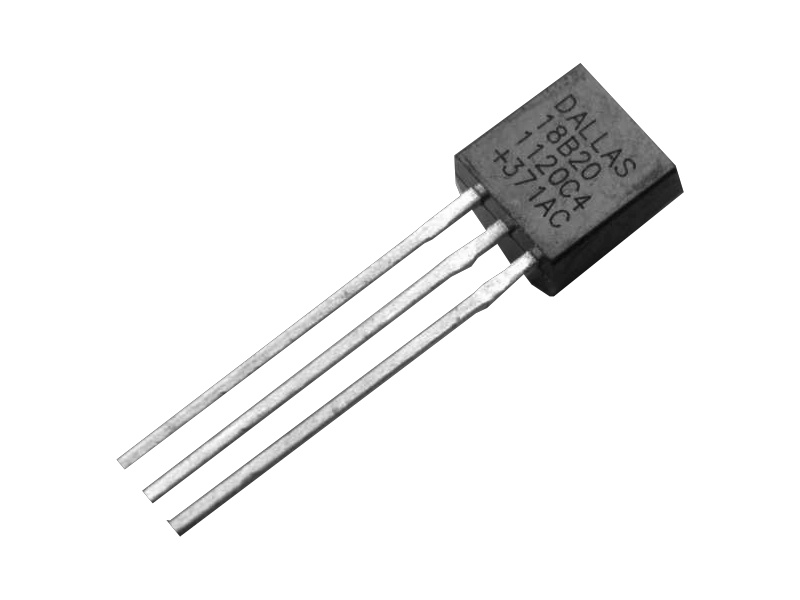
\includegraphics[width=.4\linewidth]{Figures/ds.jpg}
	\caption{DS18S20 Temperature Sensor}
	\label{fig:ds}
\end{figure}

The Arduino Due is a large Arduino, it is the first one with a 32-bit ARM core micrcontroller, has 54 digital I/O pins, 512KB flash memory, 96KB SRAM and a 84MHz clock speed. A lot of microcontrollers are 8-bit which means that they are limited in their cryptographic options. With a 32-bit architecture and a large amount of flash memory it is possible to have a light weight cryptographic library for our application but the Due is still low cost enough that it can be used for an IoT sensor application. Because it is an Arduino it benefits from the large community, wide range of compatible components and large set of open source libraries. The image shown is taken arduino.cc \cite{dueimage}.

\begin{figure}[H]
	\centering
	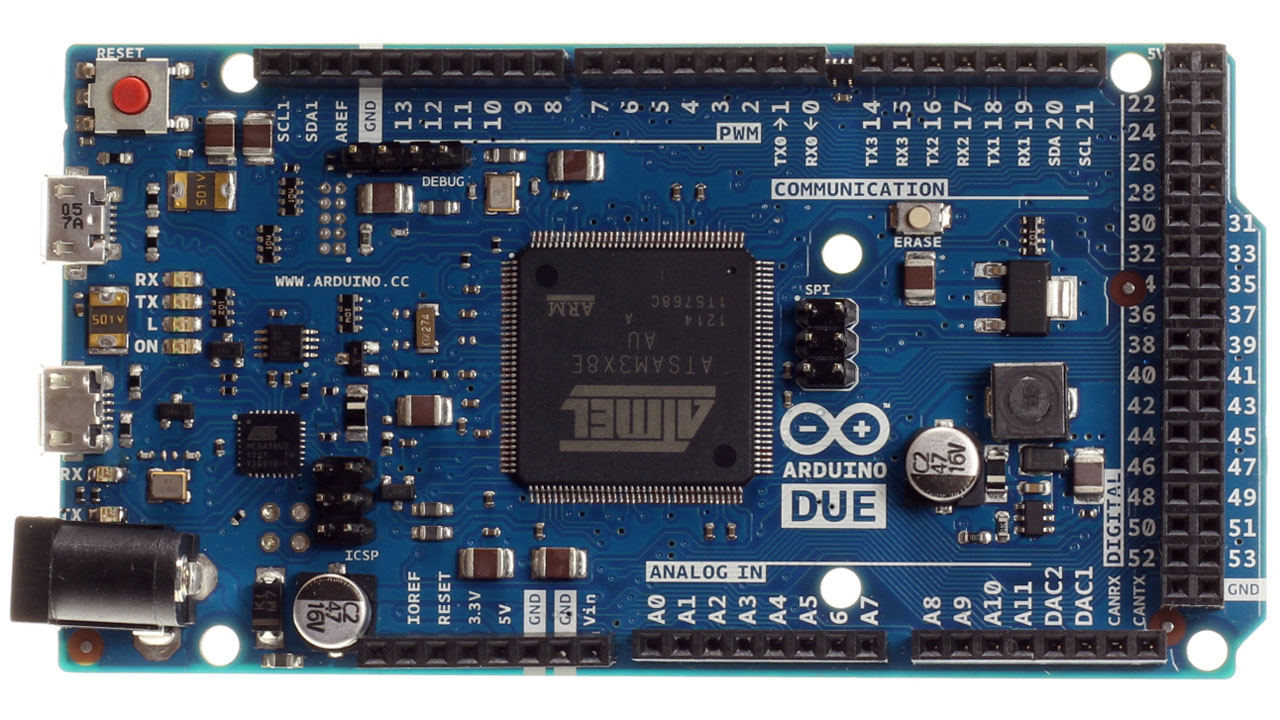
\includegraphics[width=.4\linewidth]{Figures/due.jpg}
	\caption{Arduino Due Microcontroller}
	\label{fig:due}
\end{figure}

Once the temperature data is on the microcontroller there needs to be a way to transmit the data. As the data is being sent over a network the natural choice is an Ethernet or WiFi shield. The Ethernet Shield was chosen as it is much cheaper than the WiFi Shield but completes the same job. The first revision of the shield is no longer made so the second revision, R2, will be utilised. It allows for easy connection of the Arduino to the Internet, it uses the Wiznet W5500 Ethernet chip, supports up to 8 different socket connections at a speed of 10/100Mb and has a MicroSD card slot to store network settings. It needs an different library than the first revision\cite{eth2}. Fortunately the two libraries share the same API so software that was built for the first revision is compatible with the second. Simply swap put the older shield and library and replace with the newer one. The image shown is taken from arduino.cc \cite{ethimage}.

\begin{figure}[H]
	\centering
	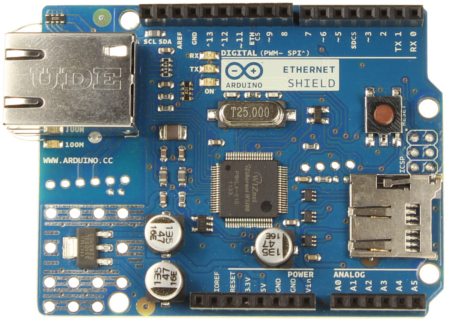
\includegraphics[width=.4\linewidth]{Figures/ethernet.jpg}
	\caption{Arduino Ethernet Shield}
	\label{fig:eth}
\end{figure}

\section{Security}

There are a lot of security options for desktop programmes and communications like AES, WEP and SSL. In this more ubiquitous field the implementations have been around for a while but for microcontrollers only in recent times have they become powerful enough at a cheap enough price and therefore popular enough for developers to write or adapt cryptographic libraries suited for microcontroller communications. The library in this application had to have acceptable security, really as close as possible to encryption systems in more powerful computers but still have acceptable performance, have a small enough code size to be stored on the microcontroller and be easy to use. Of course, it needs to prevent attackers from reading or altering the data and proving who sent it. Some microcontroller applications have extra chips that are solely for encryption but that comes at extra cost.

%Are 4-8 bit crypto libraries just not as good as 32 bit?

TweetNaCl was chosen for this project. It is a public-domain, auditable and tiny implementation of NaCl, a high-speed cryptographic library. NaCl aims for absolute performance with good security at the expense of portability whereas the aim of TweetNaCl is portability, small code size and auditability. The developers claim it is first auditable high-security cryptographic library. It is a recently created library, released in 2014 and it provides public-key cryptography, secret-key cryptography, hashing and string comparison. TweetNaCl is a full cryptography library but has only two files, needs little to no memory to be stored, has similar performance to NaCl and is easy to use. It has a set of high level methods that require the necessary variables and returns the encrypted or signed message. It doesn't provide many options, you call the method with the message and keys and the software does the rest. This reduction in customisability reduces the likely hood of a mistake by a developer using the library.


\section{Server}

\subsection{Web Server}

The web server is needed to be able to complete the relatively difficult jobs of decryption, checking signature and integrity, pulling data from the SQL database and displaying the data. For this reason and the fact that there is a Java implementation of TweetNaCl from a developer called Ian Preston, a Java Server Pages application was set up running on Apache Tomcat. JSP is a tool to dynamically create web pages using Java code. JSP could be joined with the Java implementation of the C library, TweetNaCl, to retrieve the encrypted values from a database, decrypt and display them. For the database structured query language, SQL, was chosen. When the data is being sent to the web server it needs to be sent in a particular way. Data is passed into and taken from servers is using POST and GET requests. And it is possible to send a GET or POST request to a file and that file then executes. When the Arduino is sending data to the database it was decided the script it sent a POST request to would be a PHP file as taking the encrypted and signed data and storing it could be handled by a simple PHP script.

\subsection{Arduino Server}

If it is desired that the temperature be taken from more than one location then there will need to be multiple nodes on the network. Or if there needs to be extra microcontrollers on the network for some other task. One such task is the distribution of public keys, if the server is to update it's public key, say as part of a regular update schedule to provide good security or if a key is known to be comprised then it will need a way to pass on the key. The Due can request a new key or the server can indicate to the Due that a new key has been made available and the Due will make a request for that key then make a connection to the other Arduinos in the network and send them that key. An extra Arduino Uno was chosen as an extra node for testing. The network will be built using Ethernet and be an extension of the Arduino Due to web server relationship. As the Arduino Due is a client to the web server the other nodes will need to be hosts if information is to be passed between them. The setup described in figure \ref{dia:node} is desired. 
%Chapter of Implementation
%What my app has, (how it evolved?) in terms of physical structure and technologies involved

\chapter{Implementation}
\label{imple}


\section{IoT Platform}

The basic concept of this platform is an Arduino Due that takes the current temperature of the room from a DS1820 temperature sensor. Then that data is signed and encrypted with TweetNaCL before being transmitted, using an Ethernet Shield, across to an SQL server. A web application takes the SQL data decrypts, checks the signature is valid then displays on a website. 

graphic here pls

Why was the Due chosen, 32 bit?

DS1820 is a lost cost temperature sensor that is very accurate, 12 bits of precision? and is also low power. It can scavenge power from the data with the arduino and thus does not need it's own power source. 


For the prototype, an Ethernet Shield was used as it is much cheaper than a WiFi shield but ultimately completes the same job. The shield is a simple way to connect arduinos to the internet. The shield used was the second revision, R2 and has a w500 ethernet controller. 


What are some of the options for the base station, Due/MSP430?  And for the internet connection   Ethernet?WiFi shield?

\subsection{Temperature reading}

The Due is used in two separate ways in this project; first is the client to the java web app and second is a demonstration of secure public key transmission with another Arduino Uno and Ethernet shield. The first takes the raw hex values from the DS18S20 temperature sensor, example code for this is fairly common as the Arduino can use the OneWire library which is a proprietary protocol developed by Dallas Semiconductor. In essence the command 0x44 is sent to the device using ds.write(0x44), where ds is at instance of the OneWire class,
%/cite{http://playground.arduino.cc/Learning/OneWire}
the sensor reads the internal ADC and copies the data to the scratchpad registers which can be read by sending the command 0xBE then using the command ds.read() which returns the value. Those values are put into an array which is then added to the end of an array where the first 32 bytes entries are 0x00. Then encrypted

\section{Data transmission}
The data is packaged up as a POST request
 
\section{Server Side}

For the prototype, an Apache server, SQL server and Tomcat server was set up using XAMPP on a desktop. A Java web app was created as that is the language the writer has the most experience in and there are Java implementations of the TweetNaCl library, among other variations, available. The SQL table is a simple table that holds a key, timestamp and the signed and encrypted temperature sensor. (example?). The web app upon being accessed decrypts and checks the signature of each entry, using the keys that it has stored, in the table before converting the raw hex temperature data into more readable integers and displaying in a simple HTML table that can be accessed by the user. When the Arduino has data to send it will make a POST request to a PHP file on the Apache server which takes the data given to it and places it in the SQL server. (security flaw!)

\subsection{Java web app}

The Java Web app details what the server is do when it gets various types of request, be it get or post...(more on requests?). In this type of application you can dynamically printout all the HTML that will be used to make up the page. The usual  HTML, head, body tags are printed at the top and the titles in the table are printed as well. (How it gets the keys?!). The web app uses JDBC to create a driver(idk man) to get the connection to the SQL database. Then using Java language it builds up a SQL query to take out all the values from the database and executes that. This puts all the table entries into a result set and the app cycles through that results set getting the relevant information out. The signed and encrypted hex is encoded as string and some leading zeros are lost in the conversion from byte array to string in the Arduino so these are added now before the string is converted back into a byte array. There is a try catch around the crypto\_box\_open and crypto\_sign\_open method so the server doesn't crash if one result set has been broken. Following this is the conversion from hex into integer for the user to read (how does it do it?) and finally the values are written to the browser along with the ending html tags.

\subsection{PHP}
PHP is a server-side scripting language 

There are two files in the server, connect.php and add.php. The Arduino makes a post request to the add.php which effectively just calls it and the first thing the add file does is call connect which has the server details and makes creates a connection. Following that there is a SQL query that inserts the values sent in the post request into the appropriate table entries then close the connection. cooodee snippets

\subsection{XAMPP Server}
Apache for php files, SQL and Tomcat for web app. Accessible through web by port forwarding.
what does the SQL table have?!

how does one access the xampp


\section{NaCl}

The TweetNaCl library as it stands in it's original form is not compatible with Arduinos. The C library compiles without errors but the compiler warns that the TweetNaCl method names are undefined and as a result do not perform their tasks. The method simply returns random numbers, it is possibly that it is trying to access some area of memory and simply returns whatever it finds.(ask greg/james). It is not understand why this is the case but it is a simple case of converting the library into C++ syntax. With a header file that has the main methods used in the project and the \#defines and a cpp file with the TweetNaCl code. This is added in the same way to the Arduino IDE and in the code an instance of the class is created and methods are accessed with the dot operator.

The keypair, crypto\_sign, crypto\_box and equivalent opens were used. These are simple to use, abstracted methods that make this library easy to use. For the encryption the method needs the message to be encrypted which needs to have the first 32 bytes be zero, an empty array that needs to be at least the size of the message with the leading zeros, the length of the message, the nonce, arduino public key and the servers private key. This will reveal the temperature data with the signature. To remove the signature, the crypto\_sign\_open method needs the server secret signature key and the signed cipher array.

\section{Machine to Machine}


secure M2M public key transmission
talk more about that 
%Chapter of secureness
%How safe is my app, what attacks can it stand up against and why

\chapter{Strength Of Security}
\label{stre}

%Has this become the results section??
%In the result, you simply display results, don't discuss, that's for critical evaluation

\section{Naive Sign \& Encrypt or Encrypt \& Sign}

There are problems with naive implementations of Signatures and Encryption. Both encrypting and then signing and vice versa. If a plaintext message is signed by Alice and sent to Bob encrypted with his public key. Bob can decrypt the ciphertext and re-encrypt with Charlies public key before sending it to Charlie. When Charlie decrypts the message using his private key and verifies the signature with Alices public key he finds that Alice sent the message. Charlie has been tricked by Bob into thinking Alice has sent he a message. If the opposite were to happen, if Alice sent a message to Bob that she encrypted before signing. Charlie can capture the message, strip off Alice's signature, replace with his own and take credit for the message. One assumes that Charlie knows what the message will contain. Also, by signing a cipher text it can no longer be proved that the owner of the signature was aware of the message contents. These are fairly rare edge cases but they should still be considered. It could be argued that Alice should not have trusted her first message with Bob or that an individual should never sign a cipher text because they don't know what the message contains. Or that Charlie should not assume that if he recieveds a signed message that he was defintely the intended recipient.      However, these are weak arguments as humans are not infallible, mistakes happen and there can never be a guarantee the receiver is trustworthy \cite{signencrypt}.


This application gets around those problems by using TweetNaCl's authenticated encryption as well as a signature and prepending the messages before encryption and signature with the Arduino's own unique identifier and the unique identifier of who it sent the message to. By using authenticated encryption the server can validate the message was sent by the Arduino, had not been altered in transit nor viewed by another party. After decryption the server is still able to re-encrypt with it's another party's public key and send it to them and prove that it was originally sent by the Arduino. The signature provides another layer of security as the server can prove again that the message sent by the Arduino is the same as received and it can use the two identifiers to prove that the Arduino sent it to the server. The server can't surreptitiously forward the message without changing one of the unique identifiers and therefore invalidating the signature.



%Generally encryption stops unauthorised parties from accessing information, assuming authorised parties are the only party with access to a secret key, and prove message integrity. Signatures prove that the message came from a known sender and the sender cannot deny sending the message. These are two distinct operations and the order of these operations matters. If a user was to encrypt a message then sign and send it, as the signature is added to the plain text message, it can be stripped off by an attacker. They can now use the signature to impersonated the real recipient. Signing after encryption partly defeats the purpose of signing, which is to prove that the owner of the signature saw the data and cannot disprove that they didn't send it if their signature is attached to it. If an encrypted message is signed then it is entirely possible that the owner of the signature was not aware what was in the message. In this application the message is signed first so the hash is taken of the plaintext message before being encrypted and it can be proved that the signer was aware of the message contents\cite{signencrypt}.


\section{Storing data in plaintext}

Storing vital data such as passwords and usernames in plain text in a database is generally considered quite a bad idea. This provides one point of failure that if broken means that every password stored is now useless and the accounts are wide open. In some circumstances that initial break might not seem so severe, say if that is for a forum site where the worst action that could be taken was writing an inappropriate message but users sometimes use the same password for many different sites. Although in this application the information being stored in temperature data and not passwords but the security implications are still there. This application would have that single point of failure. It is necessary to provide as many layers of security as possible rather than have one hard outer layer. That being the security of the database. As such this application stores all the temperature data as it arrives, in it's encrypted form. This way if an attacker gains access to the database they will need to know all the keys as well in order to gain the data.
%should be in hash or something better as we'd need to store all the keys and work out what key to use on what data if we ever wanted access.

\section{Public Key Transmission}

If the keys are preinstalled they can be used to sign and encrypt new public keys before they are sent. So that the receiver can use the preinstalled keys to prove integrity and authenticity of the new keys. If there are no preinstalled keys then there is no way to prove that the public key being received is indeed the public key sent. At least for a computer. The most secure and safe method to make sure the keys are the same is to have a human user manually inspected the key before sending and after sending and carefully ascertain that the one sent is correct. If there has been a man in the middle, MITM, and either the key has been altered or replaced entirely then the human user can see the difference. 

\section{Bit Flipping}

Bit flipping is the process of changing parts of the encrypted message so that it says something else. This is especially potent when the format of the message is know. As the format of the message is know to us, a test can be set that if it succeeds would change a number. In this project a test was set up to demonstrate TweetNaCl detected that the message had been altered in transit. After a message was encrypted it was altered with random hexadecimal numbers and it each time the decryption process would fail. The encryption process adds a hash of the message and the decryption process would find a different hash and would fail each time. The encrypted temperature data will not decrypt if the encrypted message has been altered and therefore won't be displayed.

\section{Timing Attacks}

TweetNaCl is an example of constant time software, which means that the time of execution does not depend on secret data and is therefore not vulnerable to timing attacks. To have this quality TweetNaCl avoids all loads from address and all branch conditions that depend on secret data and it is thus inherently protected against cache timing attacks. 

\section{Replay Attacks}

This attack is the act of resending captured valid messages to repeat a valid action, like sending money or authentication. The potential for serious damage by a replay attack here is limited. If an attacker resends some data to the server, say a malicious set of temperature data, when the server would go to decrypt that message it would try to use the incorrect nonce and public key and the message would be ignored, thus protecting the application from replay attacks.

\section{Cipher Text Characteristics}

It is possible to find out the length of the message when it is encrypted with TweetNaCl. For example if the message is a very long message in contrast to a short message there are noticeable differences. It is a vulnerability that exists in the cryptography chosen but it is a common weakness and one that does not have much consequence. Although the attacker might not know if the message was signed first, it still provides only two options for the length. If the length can be found from the cipher text is it possible for any other details to be leaked out. If the message is of a really high number, does that mean that more of the byte values are higher or conversely if it is a very low number. To test this and look at the output for different String messages, the messages were YES, NO, 0, 1 and 99999 were encrypted. 

\begin{table}[H]
	\centering
	\begin{tabular}{ | l | p{7cm} | }
	\hline
	Plaintext Message & Encrypted Message \\ \hline
	YES & 0xAE, 0x43, 0xCD, 0xA5, 0x8E, 0x54, 0xE9,  0x30, 0x59, 0xB1, 0xD5, 0xA5, 0xBF, 0x24, 0x9D, 0xEE, 0x69, 0xDB, 0x37  \\ \hline
	NO &  0x2E, 0xBC, 0xCC, 0x6B, 0x9E, 0xDB, 0x29, 0x64, 0xF6, 0x26, 0x49, 0xEF, 0xE9, 0xFA, 0xBD, 0x9C, 0x7E, 0xD1 \\ \hline
	\end{tabular}
	\caption{Resulting ciphers for encrypting words}
	\label{tab:yesno}
\end{table}

From theses message it is possible to tell the number of bytes sent if you know that the encryption method adds 16 extra bytes but other than that this test shows there isn't a discernible difference between encrypting YES and NO.

\begin{table}[H]
	\centering
	\begin{tabular}{ | l | p{7cm} | }
	\hline
	Plaintext Message & Encrypted Message \\ \hline
	0 & 0x5B, 0x74, 0x76, 0x4C, 0xF4, 0x19, 0x65, 0x37, 0xC4, 0x53, 0xAF, 0xB0, 0xCE, 0x18, 0x01, 0x01, 0x30, 0x9E \\ \hline
	1 & 0x49, 0x1B, 0x1E, 0x52, 0x10, 0x38, 0xD7, 0x38, 0x30, 0x65, 0x71, 0xBC, 0xEE, 0x65, 0x3D, 0x6, 0x31, 0x9E\\ \hline
	99999 & 0x0C, 0x0C, 0x29, 0xE2, 0x4E, 0x81, 0x67, 0x05, 0x78, 0x49, 0x8C, 0xA1, 0x4F, 0x69, 0x08, 0xBB, 0x09, 0xA7, 0x5D, 0x63, 0x4D \\ \hline
	\end{tabular}
	\caption{Resulting ciphers for encrypting numbers}
	\label{tab:9999}
\end{table}

Again, the bytes return from encrypting the test case of numbers don't indicate that the integer contained in the message is increasing in magnitude but it does show that the number is increasing in length. If the numbers were 111 and 554 the message length would be no indicator and no information would be leaked. One solution to this is to pad out the message so that it was always a set length. With a set message length a message's length would need to be the set message length or shorter. If the message was shorter then extra characters are put in to mask the true length of the message, thus messages of variable length could be sent without altering the length of the cipher text, this wasn't included to the project due to time constraints.  



%getting the encryption and decryption to have the same nonce

%Chapter of Results
%Lets see it in action
\chapter{Results}
\label{res}

The basic objectives were to sign and encrypt a message in order to stop an attacker from reading he messages and to protect against them being altered in transit. To send that message to a web server and have that data be accessible by a user.

\section{Basic Objectives}

It can be seen that the DS18S20 temperature successfully found the temperature of the room. That that data was given a signature and then encrypted. It was then packaged up and sent as a POST request across the network to a web server that stored the data in a database. Then the user could access that database and view the temperature data. The message could not be read as it was encrypted nor could it be altered as the signature verification process would fail. 

\section{Power Consumption!}

As this is to be a low power system that might run on batteries for a good amount of time, it is important to analyse the power consumption of the device. Although saving power wasn't a top priority concern in the creation application, there is more that could be done to save power such as completely shut down modules on the Arduino Due that are never used. The temperature won't be taken every second so between bursts of activity the Due could be put into a sleep mode and be woken up on an interrupt rather than the busy wait implemented in this prototype.

To start the power was recorded as the temperature was being taken with the DS18S20 temperature sensor, in both parasite power mode and regular power mode. It was found that during both operations the power consumption was the exact same at .123A and .613W. This result was not surprising as the power consumption of the temperature sensor is so small compared to the Due that even though it doesn't consume power in parasite mode, the overall consumption of power is barely affected.

To isolate the the power consumed when the Due was only signing and encrypting, the Ethernet shield was left unplugged. This way the effect of the encryption would be seen without the effects of powering an Ethernet shield throughout. 
The readings upon start up were 0.123A and 0.613W, when the data was being given a signature the readings were .17A and .970W and when the message was encrypted it rose to .20A and 1W. 

In addition the power consumption when the Ethernet shield was attached but had no cable plugged was recorded. The power consumed during the signature and encryption process was the same as above but during DCHP the readings were .199A and 0.990W as it tried to gain an IP address from the router. Once the loop iteration was complete, the code went straight into a busy loop which was a tiny drop in power at .198A and 980mW. A busy wait is a waste of power and resources so at this point the Arduino Due should go into a sleep mode and be woken up by an interrupt when it was to record the temperature again. 

The next test was with the shield plugged into the router with the Ethernet cable. The power consumption shot up to 0.265a and 1.30W during DHCP at the start of the sketch and there it remained even during the encryption process. Evidently the shield requires such a significant of the power that by comparison the cryptographic library is as good as unnoticeable. There are versions of the Ethernet Shield with an extra module that allows power over Ethernet. This extra module doesn't add a significant increase to the overall cost to the shield but can alleviate battery problems and extend the life of batteries by extracting power from the Ethernet cable that is connected to the router
%voltage changes??

The final test was to find out if there was a difference in power consumption depending on the length of message sent. Messages of size 20 and size 250 were sent with no appreciable difference in power consumption found.


The voltage through the experiments was the exact same, a steady 4.96V which makes sense as this is round about what USB 2.0 can give out and is well within normal limits for the Arduino Due.


%is flashed the normal way
%take temp reading every couple of seconds in parasite mode, 
%4.96V, 0.123A, 613mW
%flashed through device with empty code
%power reading stay same
%flashed normally with empty code
%same
%flashed normal and not
%take temp reading every couple of seconds in parasite mode
%same again
%During the dhcp and connecting to server .199A and 990mW with no ethernet plugged in
%During the busy wait at the end of loop delay() the current is .198A and 980mW a tiny drop in current
%with ethernet plugged in, sending encrypted data
%1.30w /0.265a
%tested on data of 19 length and 209, made no difference
%with ethernet plugged in but no encryption
%1.30w /0.265a


\section{Additional Objective}

\subsection{Secure transmission of public keys}

Expansion of the network was considered with multiple devices communicating directly. This objective was reached by adding an Arduino Uno with another Ethernet shield as a webserver and the Due could pass on data, such as new server public keys, to it. If more nodes where desired then more Uno webservers could be added and the Due would simply go through the list of servers and send a POST request to each to update their keys.

show lots of pictures?

\subsection{rekeying on arduino}
%http://blog.skylable.com/2014/05/tweetnacl-carrybit-bug/
%Chapter of Critical Evaluation
%What is maybe not so great about it
\chapter{Critical Evaluation}
\label{crit}



With the way it is set up at the moment the XAMPP server pages, add.php and connect.php, and the JSP application that displays the temperature data are accessible through a browser by anyone on the network. Realms could be set up or IP filtering. A realm is a database of usernames and passwords that identify valid users of a web app and can be used to provided levels of access.

%The way the arduino accesses the new server public key at the moment is simply by sending a GET request to the server for it. But an attacker could easily send the same get request and get a public key. Then this key could be used to send mesages to the arduino causing damage at worst or at least the server and arduino might be out of sync and each are using a different set of keys and be unable to read communications from each other.

The public and private key of the server and the public key of the arduino are stored as plaintext in the web application and it might be possible to read them from the WAR files. This is not as much a problem for the public keys, if caught quickly, as it means we can no longer trust that new messages are from an authorised source but if the secret key is leak then all messages sent from the Arduino using that key pair are compromised. 

The messages are padded with zeros to avoid leaking out the message length. Perhaps it would be better to include random data rather than a set of never changing zeros. Thus the rare case that an attacker notices that the first 32 bytes don't change or worse that they are all the same would be avoided.

The Arduino doesn't have access to /dev/random and can't provide good enough random data to make good key pairs. Which means that it can't update it's own secret key, for example if the key has been compromised or it is part of a regular renewal service to key security tight.

When the public keys are transmitted for the first time, a human user is required to manually inspect the keys, in private, and ensure they are the same before they can be used for data transmission. This is, unfortunately, unavoidable as there is no way to prove that this key that arrived is the one that was sent. The internet is an unsecure platform and it cannot be trusted. There are many things that could happen as it transits the web. 

The PHP files that the Arduino Due sends a POST request to do not authenticate the requests and as such anyone who knew the ip address of the server could send data into the SQL database. However when the Java web app retrieves the data out of the database if it is not encrypted with the keys then the decryption will fail and the data won't be displayed to the user.

The JSP page that sends a new public key and encrypted nonce to the Arduino Due does not have any restrictions on it's access. Therefore is a malicious connection is made to the server then that connection will receive the data. This public key and nonce could then be used by the attacker to add in their own data or to simply interfere with the normal operation of the application. This could be solved in a similar manner to securing the PHP files with IP filtering or setting up a realm.

If a encrypted temperature message doesnt make it, then the sync is lost

Generally not a good idea to store things sequentially

This prototype has used the Ethernet Shield as it was much cheaper than a WiFi shield. If an implementation similar to the one described in this report was to be implemented then it would be convenient to provide connection over WiFi. The product also risks not being adopted as more and more products have wireless capabilities and  users see it as the norm and resent cables. This will be especially important if the device uses batteries to power itself.

%Chapter of Conclusion

% Review and summarise points
% What do I want the reader to come away with - Security is important, can be easy with a small amount of fuss, can be done on IoT, why arduinos are good and 
% how they will help encryption on small systems as they are affordable but powerful, how important IoT will be 

% design/feasability report
% Major conclusion
% Reference to aims and objectives then advantages of findings
% support for choice
% authors evaluation

% feasability/recommendation report
% background to problem
% research problem
% major conclusion
% support of conclusion
\chapter{Conclusion}
\label{conc}

This report has shown that is it possible to provide low power, not overly complicated encryption and authentication on a micrcontroller based IoT system. TweetNaCl is an excellent library that can be added to any project easily, has tiny code size but still provides acceptably strong encryption at a quick speed. It is a full library and can produce asymmetric and symmetric encryptions plus a SHA-512 hashing function and a string comparison function which any system can implement to cover it's encryption needs.

In any computer application which handles information that is private and/or could be used to do damage such as a persons credit card details meaning that person loses money or the lose of private user data that causes the loss of trust and damage to the reputation of a company, needs good encryption. As more and more devices are connected to the internet such, as smartphones, smart televisions, smart domestic appliances and anything else an IoT engineer thinks might benefit from an internet connection. As the entire planet shifts more and more into the digital world, this need grows ever larger. When data, such as credit card details, are lost this may be a huge problem but it is not fatal. However with the advent of heavy machinery such as cars becoming part of the internet of things, and other examples no doubt soon to follow, security should be at the forefront of everyone's minds. This project has aimed to show that acceptable encryption can be implemented easily, even on low power systems. In the prototype the users private temperature data is safe from attackers. 

Arduino too, was a good choice as Arduinos have been use for fast prototyping and for teaching people who might not have a background in electronics or computing how to create projects, such as IoT projects. There a multitude of internet connected projects for the Arduino, many connect to benign objects such as the LEDs on the board but they can be connected to many more things, some which can be troublesome if compromised. Security is generally an after though, for experienced and novice developers alike. Even massive companies with millions pounds worth of revenue make security blunders or just don't bothered. It is hoped that this project will add to the list of secure, internet connected Arduino projects available so that one of the first things of everyone's mind when starting a project is security. The powerful but lost cost Arduino devices prove that it is possible to have good quality security in any IoT system and more security options will pop up as the price to performance ratio continues on it's upward trajectory. Which is very beneficial to the IoT industry as a whole.

Security measures will never be fully secure. Given infinite computer resources and infinite time any security algorithm can be hacked and there might bugs, backdoors, employees willing to leak secret keys. However if the algorithms make it unfeasible to attack or simply not worth the attackers effort required then that is as good as fully secure. At the moment there are so many devices that simply have no protection that there is an open source project google powered search engine that shows all the devices that are vulnerable. These devices lack even rudimentary security features and even a casual attacker with not too much knowledge or experience could gain access and control. By having even the minimal amount of protection, obviously the more protection the better, you can dissuade would be attackers because they have plenty of easier targets. Or make it so that the reward of breaking into your system simply is not worth the effort.

The TweetNaCl library satisfies all the requirements of a good microcontroller cryptolibrary. It is open source and the developers encourage it's use where ever possible. It was used with success in this project as the users private data could not be read in transit nor altered in transit and the receiver could prove that a certain person sent the message. 
 
%\include{ further work }

%----------------------------------------------------------------------------------------
%	THESIS CONTENT - APPENDICES
%----------------------------------------------------------------------------------------

\appendix % Cue to tell LaTeX that the following "chapters" are Appendices

% Include the appendices of the thesis as separate files from the Appendices folder
% Uncomment the lines as you write the Appendices

% Appendix A

\chapter{Appendix Title Here} % Main appendix title

\label{AppendixA} % For referencing this appendix elsewhere, use \ref{AppendixA}

Write your Appendix content here.
%\include{Appendices/AppendixB}
%\include{Appendices/AppendixC}

%----------------------------------------------------------------------------------------
%	BIBLIOGRAPHY
%----------------------------------------------------------------------------------------
%\bibliographystyle{plain}

%need to compile bib.bib
%then run bibtex main.aux
\printbibliography

%\begin{thebibliography}{99}
%\bibitem{lamport}
 % Leslie Lamport,
  %\emph{\LaTeX: a document preparation system},
  %Addison Wesley, Massachusetts,
  %2nd edition,
  %1994.
%\end{thebibliography}


%----------------------------------------------------------------------------------------

\end{document}  
